\documentclass{article}

\usepackage[utf8]{inputenc}
\date{}
\usepackage{amsthm,amssymb,amsmath}
\usepackage{graphicx}
\graphicspath{ {./images/} }



\newcommand{\NN}{\mathbb{N}}
\newcommand{\ZZ}{\mathbb{Z}}
\newcommand{\RR}{\mathbb{R}}
\newcommand{\QQ}{\mathbb{Q}}
\newcommand{\CC}{\mathbb{C}}
\newtheorem{theorem}{Theorem}[section]
\newtheorem{corollary}{Corollary}[theorem]
\newtheorem{lemma}[theorem]{Lemma}
\newtheorem{proposition}[theorem]{Proposition}
\newtheorem{conjecture}{Conjecture}
\newtheorem{definition}{Definition}
\theoremstyle{remark}
\newtheorem{example}{Example}
\newtheorem{answer}{Answer}
\newtheorem{remark}[example]{Remark}

\title{ODE with Lipschitz Coefficients Draft 2}
\author{Phillip Yan}


\begin{document}

\maketitle

%%%%%%%%%%%%%%%%%%%%%%%%%%%%%%%%%%%%%%%%%%%%%%%%%%%%%%%%%%%%%%%%%%%%%%%%%%%%%%


\section{Introduction to ODEs}
To prove the existence and uniqueness of solutions to ODEs with Lipschitz coefficients, let us first introduce Ordinary Differential Equations. \\

\subsection{Solving ODEs and Examples}

A key concept in math that appears often in the real world is the idea of a rate of change. Readers may already be familiar with the derivative from Calculus as a measure of a rate of change of a function. Sometimes, it is easier to consider the rate of change rather than the absolute amount of change.

A clear real world example can be seen in the expression of acceleration as the change in velocity. That is, 

$$v'(t) = a(t),$$

where $v'(t)$ is the change in velocity at a given moment of time t, and $a(t)$ is a function for acceleration at time t. Here, in the absence of a clear function of velocity, we see the change of velocity expressed as a function of acceleration. Similarly within physics, it is possible to model the motion of a pendulum with the following differential equation. Given $\theta$ as the angular displacement, $L$ as the length, $g$ as the constant for acceleration due to gravity, we have the following equation: \\


$$\frac{d^2\theta}{dt^2}  = - \frac{g}{L}\sin{\theta}.$$

Note that similarly, the function directly relating angular displacement with time is unknown; here, all that is given is a function that determines the acceleration of the pendulum.

Both of these equations are examples differential equations which are defined as the following.
\begin{definition} An equation containing the derivatives of one or more unknown functions with respect to one or more independent variables is said to be a differential equation.
\end{definition}

There are many different types of differential equations. A special kind of differential equation that will be the focus of this paper is the Ordinary Differential Equation.

\begin{definition}
    A differential equation that contains derivatives with respect to a single independent variable is called an ordinary differential equation (ODE).
\end{definition}

For this paper, we  will consider first-order ODEs as higher order ODEs can be turned into first-order ODEs as we will show later. An example of a first order ODE is:
$$y'(x) = f(x,y).$$

Intuitively, like all differential equations, an ODE is a representation of a rate of change. In this particular case, the derivative of a function, $y'(x)$, is expressed in terms of a function of $x$ and $y$ itself. \\

Because a function relating the dependent variable, $y$, with $x$ is not given, one may wish to ``solve" the ODE, or to find the unknown function(s) of $y=f(x)$. In the acceleration example above, it would be to determine the velocity function as based of the time variable $t$. \\

ODEs are often solved via an \textbf{initial value problem}. An initial value problem includes an ODE alongside an initial value $(x_0, y_0)$ such that $y_0 = f(x_0)$. For example, returning to our pendulum example, an initial value might be $\theta(0) = \pi$, meaning the angular displacement at time 0 is $\pi$. Thus, one can intuitively reason that a different initial value can result in a different solution. In this case, dropping a pendulum at different angular displacements can impact the resulting solution which is the function that relates angular displacement with time elapsed. \\


A solution to an initial value problem is a function $y(x)$ which satisfies the both the ODE and the given initial value $y_0 = f(x_0)$. Sometimes, there is a unique solution to an initial value problem.\\

\begin{example}

 In the acceleration example, if one is given a starting velocity at time 0, $y(0) = 5m/s$ alongside the ODE describing acceleration or the rate of change of velocity, intuitively it makes sense that one could determine velocity at any given point of time $t>0$. For ODEs of the form $y'(t) = f(t)$ one can simply integrate both sides of the ODE in a method called \textbf{direct integration}. 

$$y(t) = \int_0^tf(s)ds + y_0.$$
Note that this satisfies the initial value $y_0 = f(x_0)$. 

\end{example}

When one can separate variables in the given equation, it is also possible to use a more complex method of solving ODEs is \textbf{separation of variables}. 

\begin{example}
Given an ODE which defines $y'$ in terms of both $y$ and $x$ values for some ODE:

$$ \frac{dy}{dx} = 10xy, \quad y(0) = 1.$$

We can solve this with separation of variables because we can isolate the two variables on either side of the equation. 

Refactoring the expression to
$$  \frac{dy}{y} = 10xdx,$$

we can take the integral of both sides to solve the ODE:

\begin{align*}
\frac{dy}{y} &= 10xdx\\
\ln y  &= 5x^2 + C\\
y &= e^{5x^2 + C}, C=0.\\
\end{align*}
\end{example}

\subsection{Existence}
Although there are many other methods to solve ODEs, as ODEs get more complex, the solution might not be immediately obvious. Sometimes they might not even exist. 

\begin{example}
An example of an ODE where the solution does not exist is 
$$ y'(x) = \begin{cases} 
      \frac{1}{x} & x \neq 0 \\
      0 & x= 0 \\
   \end{cases} , \quad y(0) = 0.$$

If we $y$ is differentiable at 0, then we know  $y'(0) = 0$ and that $y$ would be continuous at 0. However, considering values $x > 0$ attempting to evaluate via direct integration we obtain the following equation:
$$y(x) = \ln x +C$$

Note that by definition of a natural logarithm:

$$\lim_{x \to 0} \ln x \neq 0$$

Therefore, because $x$ does not converge to 0, $y$ is not continuous at 0, meaning that there does not exist any continuously differential function $y$ such that $y$ satisfies the ODE and the initial condition. 
\end{example}

\subsection{Uniqueness}
At the same time, it is important to determine whether solutions are unique given a specific initial condition. In other words, we want to make sure that there is no randomness in output (the solutions) given a repeated input (the ODE). This is important in fields like physics which are deterministic. Returning again to our velocity and acceleration example, we wouldn't want two different velocity functions as our solution for the ODE and initial value problem. (You might end up with two different velocity values at a given time with the exact same acceleration and starting velocity, meaning you'll never know for certain what the  velocity is at any given moment!) \\

\begin{example} An example of an ODE where the solution is not unique is:

$$y'(x) = \sqrt{|y|}, \quad y(0) = 0.$$


Let us consider the two cases where $y>0$ and where $y<0$.

\textbf{Case 1 $(y>0)$}:
Evaluating this ODE via separation of variables and then direct integration, we see
\begin{align*}
y^{-\frac{1}{2}}\frac{dy}{dx} &= 1 \\
\int y^{-\frac{1}{2}}dy &= \int dx \\
2y^{\frac{1}{2}} &= x +C.
\end{align*}

Since we know via the initial value that $y(0) = 0$, we know that $C = 0$.

Thus, a solution is $y = \frac{x^2}{4}$.\\


\textbf{Case 2 $(y<0)$}:
Following the same process, except for $-y$, we get:
$$ 2(-y^{\frac{1}{2}}) = x.$$
Thus another solution is $y = -\frac{x^2}{4}$.




Furthermore, note that the tautological function $y = 0$ also is a solution. Although the solution to this same ODE but with a different initial condition might be unique, with the specific initial condition set by this initial value problem, $y(0) = 0$, there are three potential solution functions that satisfy the IVP.

\textbf{Not sure if this is what you mean by talking about the three function.}

We have the opposite problem as the previous ODE which had no solutions. This paper seeks to address the conditions that need to be satisfied so that there is exactly 1 solution.

\end{example}

\subsection{Example ODE With a Unique Solution}
Consider the ODE:
$$y'(x)= y^2 + xy + x^2, \quad y(0) = 0.$$

As a slightly more complex differential equation, it is not immediately obvious whether a solution exists and if that solution is unique. One can't easily separate the variables and directly integrate. Thus, for differential equations like these, we need some general theorem to assert that a solution exists and is unique.\\

In fact, we will see that this is a solvable ODE with a unique solution.


\subsection{Graphical Intuition}
Graphical intuition on the $xy$-plane might be helpful for our following discussion. Instead of a traditional graph of a function $y = f(x)$ which maps values of $x$ to values of $y$, we consider a slope field on the $xy$-plane. At every point $(x,y)$, the slope $\frac{dy}{dx}$ is calculated as a function of $x$ and $y$ and plotted on the graph to produce a field of different ``slopes" at all points in the graph. 

\begin{center}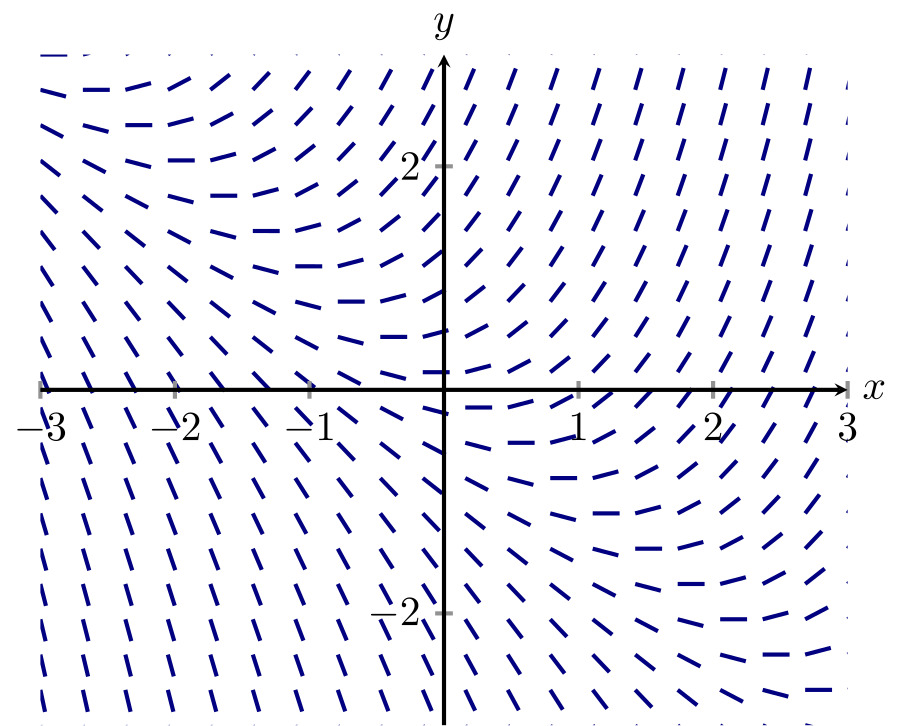
\includegraphics[width=7cm]{SlopeFieldMath.png} \\ A slope field for section 1.4 ODE ($y'(x)= y^2 + xy + x^2, y(0) = 0$) with the solution to the  initial value problem overlaid. \end{center}


Intuitively, when considering an initial value problem, one can potentially consider the initial coordinate pair given to be the coordinate of a boat, and the slope at any given point a current. Moving in the direction of the current, the ``boat" traces out a curve which is the function that is the solution if it exists to the ODE. \\


This intuition can help to serve as the basis to understand our approach in the following sections as it provides a visual basis for understanding the function $y'(x) = f(x,y(x)) + y_0$.



\section{Lipschitz Continuity}
In this paper, we will prove that such solutions exist locally and are locally unique given that the ODE is Lipschitz continuous on a specified set.

Our first step in understanding when solutions exist and are unique in ODEs is to introduce a stronger form of continuity than our previous epsilon-delta definition of general continuity.

We first introduce the concept of \textbf{metric spaces}, of which $\mathbb{R}$ is an example which we have used in class. \\

\begin{definition}
 A metric space $(X, d_X)$ is a set $(X)$ with a function $(d_X)$ defined as:

$$d_X: X \times X \to \Bbb [0, \infty )$$

such that $d_X$ satisfies the following three axioms given $x_1, x_2, x_3 \in X$:

\end{definition}
\begin{align*}
1.& \quad \text{The distance from a point to itself is 0: }d_X(x_1, x_1) = 0 \\ 
2.& \quad \text{Symmetry: } d_X(x_1, x_2) = d_X(x_2, x_1)\\
3.& \quad \text{The Triangle Inequality: }d_X(x_1, x_3) \leq  d_X(x_1, x_2) + d_X(x_2, x_3).
\end{align*}
\begin{example}
An example is the real vector space $\mathbb{R}^3$ equipped with absolute difference as the distance function: $d(x,y) = \|x-y\|$. It is straightforward to confirm that the absolute difference meets the above requirements for the distance function in a metric space given our understanding of absolute value on a number line.
\end{example}

We now can now define Lipschitz continuity: \\ 

\begin{definition} 
Lipschitz Continuity: Given two metric spaces $(X, d_X)$ and $(Y, x_Y)$, a function $f: X \to Y$ is considered \textbf{Lipschitz continuous} if there exists $K \in [0, \infty)$ such that for all $x_1, x_2 \in X$,
$$d_Y(f(x_1),f(x_2)) \leq Kd_X(x_1,x_2).$$
\end{definition} 

Intuitively, a function is Lipschitz continuous over a certain interval if there exists a set constant value $K$ that bounds the magnitude of the derivative at any point within the interval. Visually, at every point there exists a ``double triangle" made from the two lines $y = K$ and $y = -K$ such that  the graph remains outside the triangle.\\

\begin{center}\includegraphics[width=7cm]{LipschitzContinuity.png} \\ A visual representation of the ``double" trianges used to determine Lipschitz continuity at the point $x = 0.5$. Note that the absence of the curve in the white triangles represents the fact that the derivative at 0.5 is bounded by K. \end{center}
\begin{example}
A clear example of a function that is Lipschitz continuous is $f: X \to Y, y =  f(x) = x$. With the distance functions of the two metric spaces $(X = \Bbb R, d_X)$ and $(Y = \Bbb R, d_Y)$ both being the absolute difference, given two points $x_1, x_2 \in X$:
$$d_X(x_1 - x_2) = |x_1 - x_2| = |f(x_1) - f(x_2)|.$$

Thus, we know given any $K \geq 1$, $ |f(x_1) - f(x_2)| \leq K|x_1 - x_2|$ which satisfies the requirements of Lipschitz continuity.
\end{example}

\begin{example} 
A counter example can be seen in the function $f: X \to Y, y =  f(x) = \sqrt{|x|}$ on the interval $(-\epsilon, \epsilon)$. Let us refactor our definition of Lipschitz continuous to: 

$$ \frac{d_Y(f(x_1), f(x_2))}{d_X(x_1, x_2)} \leq K.$$

 Setting $x_1 = 0$ and given the absolute difference as the distance function, we see that this is the same as:

$$ \frac{|\sqrt{x_2} - 0|}{|x_2 - 0|} \leq K.$$

In order for this function to be Lipschitz continuous, the above must be true for all $x_2 \in (-\epsilon, \epsilon) $. However, note that as $x_2$ approaches 0 from the right hand side, the following occurs:

$$\lim_{x_2 \to 0}\frac{|\sqrt{x_2} - 0|}{|x_2 - 0|} = \lim_{x_2 \to 0}\frac{\sqrt{x_2}}{x_2} = \frac{1}{x_2} = \infty.$$

Therefore, because there does not exist a fixed $K$ that is greater than infinity, this function is not Lipschitz continuous on the interval $(-\epsilon, \epsilon)$ and therefore the function in general is not Lipschitz continuous on $\Bbb R$.
\end{example}


To see the relationship between this type of continuity and our more familiar epsilon-delta definition for uniform continuity, we can use the following proposition.\\

\begin{proposition}If a function is Lipschitz continuous over domain D, then it is also uniformly continuous over D.\\
\end{proposition}

\begin{proof} We will use an epsilon-delta proof. Because the function is Lipschitz, we know that for all values $x_1, x_2$ on this domain there exists a K such that:

$$d_Y(f(x_1),f(x_2)) \leq Kd_X(x_1,x_2).$$

Given an arbitrary point $x_0 \in D$ and arbitrary $\epsilon >0$, we set our $\delta = \frac{\epsilon}{K}$. Thus, any value $x$ in the domain such that $d_X(x_1,x_2)<\delta$ means also that:
$$d_X(x_1,x_2)<\frac{\epsilon}{K} \implies Kd_X(x_1,x_2)<\epsilon$$
By definition of Lipschitz continuity, $d_Y(f(x_1),f(x_2)) \leq Kd_X(x_1,x_2)$, so \\

$d_Y(f(x_1),f(x_2)) \leq Kd_X(x_1,x_2) < \epsilon \implies d_Y(f(x_1),f(x_2))< \epsilon$

\end{proof}

At the same time Lipschitz continuity is actually stricter that general continuity since it bounds the derivative. \\

\begin{corollary} 
The set of functions that are Lipschitz continuous is a subset of functions that are uniformly continuous.
\end{corollary}

We can see this through example functions such as $e^x$ on $\mathbb{R}$ or $\sqrt{\|x\|}$ on $[-1,1] \in \mathbb{R}$ where although the function might be uniformly continuous, the derivative is unbounded on the given domain. For example, for $e^x$ there does not exist a constant K such that: $$\frac{d_Y(f(x_1),f(x_2))}{d_X(x_1, x_2)} \leq K$$
where $x_1 = 0$ and as $x_2 \to \infty$ since $f(x_2)$ increases at a rate without bound. \\


The key idea here and across Lipschitz continuity as a whole is the importance of the coefficient $K$ and the importance of satisfying such a requirement in order to be considered Lipschitz continuous. The particular case when $K < 1$ also has special significance. \\

\begin{definition}A \textbf{Contraction Map} is defined on a metric space $(X, d_X)$ as a function $f: X \to X$ where there exists a real number $k, 0\leq k<1$ such that for all $x_1, x_2$

$$d_Y(f(x_1),f(x_2)) \leq kd_X(x_1,x_2).$$

\end{definition}

A contraction map is therefore an example of a function that is Lipschitz continuous and therefore uniformly continuous, as shown in Corollary 2.1.1. The smallest value $k$ that satisfies this expression can therefore be seen as the Lipschitz coefficient for the function. \\

Intuitively, the distance between $f(x_1), f(x_2)$ is smaller than the distance between $x_1, x_2$ when this map is applied. Because a contraction map is a map from a metric space to itself, one can apply this map iteratively, with each iteration contracting the distance. Eventually, intuitively, it would make sense for the points to potentially converge to a single point. 

Let us consider the following function:
$$f(x) = x^2, x \in (-1,1) \in \mathbb{R}$$

This function is Lipschitz continuous on that given interval as there clearly exists some value $K$ (say, $K=10$, or 100, or 1000 etc for clarity) that bounds the derivative $2x, -1<x<1$. At the same time, the given domain of values $|x| < 1$ implies that $x^2 < |x|$. Eventually, one could intuit that the function might converge to 0. \\

We shall prove this idea of convergence in the following generalized Banach Fixed Point Theorem in the next section.\\ 

\section{Banach Fixed Point Theorem}

Although in class we proved a version of the Banach Fixed Point Theorem, it required an assumption of a compact metric space. Here instead we shall prove a theorem with only the assumption of a complete metric space. We first need the following definitions\\

\begin{definition} A sequence defined on a metric space $(X, d_X)$ is Cauchy if for all $\epsilon \in \Bbb R, \epsilon > 0$, there exists a positive integer N such that for all positive integers $m, n >N $ 

$$d_X(x_m, x_n) < \epsilon$$

where $x_m, x_n \in X.$
\end{definition}


We will use this definition of a Cauchy sequence in defining a complete metric space as follows.

\begin{definition} A complete metric space $(X, d_X)$ is defined as metric space where all Cauchy sequences of points in $X$ converges to a limit also in $X$. 
\end{definition}

\begin{example}
An example of a complete metric space is $\Bbb R$ equipped with the absolute difference as the distance function.

We know that a Cauchy sequence of real numbers is bounded on $\Bbb R$, which means by the Monotone Convergence Lemma that proved in Honors B, we therefore know that every Cauchy sequence converges on that metric space.
\end{example}

\begin{example}
An example of an incomplete metric space is $\Bbb Q$ equipped with the absolute difference as the distance function.
\textbf{Not sure I would need to prove this and the previous example}
\end{example}

Now we can express the Banach Fixed Point Theorem.\\

\begin{theorem} \textbf{Banach's Fixed Point Theorem:} Given a complete metric space $(X, d_X)$ and a contraction mapping on $X$ defined as $T: X \to X$, there exists some unique fixed point $x \in X$ such that $T(x) = x$. 
\end{theorem}

\begin{proof}
We shall approach this proof in three steps. \\
\textbf{Part 1: }First, we will prove that such a sequence defined by the contraction mapping

$$x_0 = x_0, x_1 = T(x_0), x_2 = T(x_1), ... x_n = T(x_{n-1})$$

for some arbitrary initial value $x_0$ is Cauchy. 
Let us now find a relationship between the distance between any two adjacent elements in a sequence with the distance between the first two points. By definition of the above map, we can define the distance between two adjacent elements $x_{n+1}, x_{n}$ as
$$d(x_{n+1} , x_{n}) = d(T(x_{n}) , T(x_{n-1})).$$
By the definition of a contraction map, we know that there exists some K such that

$$d(T(x_{n+1}) , T(x_{n})) \leq Kd(x_{n}, x_{n-1}) $$

Iterating the above step, we see that:

$$d(x_{n+1} , x_{n}) \leq Kd(x_{n}, x_{n-1}) \leq K^2d(x_{n-1}, x_{n-2}) \leq ... \leq  K^{n}(x_{1}, x_{0}). $$
Inductively, therefore we can use the relationship:

$$d(x_{n+1} , x_{n}) \leq K^{n}d(x_{1}, x_{0}). $$

Because all distance values are by definition positive and we know $K$ to be between 0 and 1, we can use the triangle inequality which tells us that for any $m \geq n$:

$$d(x_{n} , x_{m}) \leq d(x_n, x_{n+1}) + d(x_{n+1}, x_{n+2}) + d(x_{n+2}, x_{n+3}) +  ... + d(x_{m-1}, x_{m}).$$

Substituting the values for each of the distance measurements, we obtain:

$$ \leq (K^n + K^{n+1} + ... + K^{m-1})d(x_1, x_0) = K^n(1+ K + K^2 + ... + K^{m-n-1})d(x_1, x_0).$$

Note that since $K$ is a positive value, we know it to be strictly less than the geometric series which itself is defined to be less than or equal to $\frac{K^n}{1-k}$:
$$ < K^n(1+ K + K^2 + ... )d(x_1, x_0) \leq \frac{K^n}{1-K}d(x_1, x_0).$$

Because the limit of $\frac{K^n}{1-K}$ as K approaches infinity is 0, we can see that for all $\epsilon$ a sufficiently large n means that all values $n_0$ greater than n result in 

$$\frac{K^{n_0}}{1-K}d(x_1, x_0) \leq \epsilon.$$

Thus, we have shown that this sequence is Cauchy. At the same time, because the metric space is defined as a complete metric space, we know that all Cauchy sequences converge. Thus, there exists some point $x_{\alpha}$ in $X$ such that this sequence (let's call it $x_n$) converges to $x_{\alpha}$, or $$x_n \to x_{\alpha}.$$

\textbf{Part 2:} We now prove that this limit is indeed a fixed point
Returning to the fact $x_{n} = T(x_{n-1})$, we have already shown that when taking the limit of $x_{n}$ as n approaches infinity, we obtain $\lim_{n \to \infty} = x_{\alpha}$ for some value x that the sequence $x_n$ converges to. Thus,

$$x_{\alpha} = \lim_{n \to \infty} T(x_{n-1}).$$

Since T is Lipschitz continuous because it is a contraction map, we know from Proposition 1 that T is also continuous. Therefore, we can move the limit into the function to obtain:


$$ T(\lim_{n \to \infty}(x_{n-1})) = T(x_{\alpha}).$$

Thus, we have shown that $x_\alpha = T(x_\alpha)$.\\

\textbf{Part 3:} Our last step is to show that such a fixed point is unique. We will prove this with a proof by contradiction. Assume that there exists another distinct fixed point $y_{\alpha} \in X$. Then, $y_{\alpha} = T(y_{\alpha})$.

We know that the distance between the image of each point after applying the contraction mapping is strictly less than the distance between the two fixed points. That is,

$$d(T(x_{\alpha}), T(y_{\alpha})) \leq Kd(x_{\alpha}, y_{\alpha}).$$



However, given the definition of fixed points, this also means

$$d(x_{\alpha}, y_{\alpha}) \leq Kd(x_{\alpha}, y_{\alpha})$$
which is impossible as with K  strictly less than 1, $d(x_{\alpha}, y_{\alpha})$ should instead be greater than $Kd(x_{\alpha}, y_{\alpha})$. Thus, the two distinct points do not exist, and $d(x_{\alpha}, y_{\alpha})$ is necessarily 0.

In these three steps, we have shown that such a unique point exists given a contraction mapping on a metric space.

\end{proof}


This proof directly results in a useful Corollary.  \\
\begin{corollary} If X is a complete metric space and $T: X \to X$ is a contraction map, for any $x_0 \in X$, $x_\alpha = \lim_{n \to \infty}T^n(x_0)$ is the unique fixed point of T.
\end{corollary}

This will serve as an abstract basis for understanding Picard Iteration.

\section{Picard-Lindelöf Theorem}
Here we will finally integrate our discussion regarding Lipschitz Continuity and the Banach Fixed Point Theorem to produce a general theorem which dictates the conditions required for an ODE to have a locally existing solution that is also locally unique.




\begin{theorem}If a function $f(x,y(x))$ is continuous with respect to $x$ and Lipschitz continuous with respect to $y$ in an open rectangle
$$R = \{(x,y)\mid x_0-a\leq x \leq x_0+a \text{ and } y_0-b\leq y\leq y_0+b\}, (x_0, y_0) \in R$$
then the initial value problem 

$$y'(x) = f(x,y), \quad y(x_0) = y_0$$

has a unique solution on some open sub-interval of $[x_0-a, x_0+a]$.
\end{theorem}

Note that for the example ODE in section 1.4, $f(x,y) = y^2 +xy + x^2$ is continuous, which by Corollary 2.1.1 means that the function is Lipschitz with regard to $y$. Thus, with the hypothesis satisfied, and with $x_0 = 0$, there exists some $a$ such that there is a unique solution on some subset of $[-a, a]$.










\begin{proof}

Given such an initial value problem, we know that we can rewrite

$$y'(x) = f(x,y), \quad y(x_0) = y_0$$

via integrating both sides in order to obtain:

$$ y(x) = y(x_0) + \int_{x_0}^{x}f(t,y(t))dt.$$


Let us consider a metric space $C$ defined as the set of continuous functions $f: [x_0 -a, x_0+a] \to [y_0 -b, y_0 +b]$ with distance function defined as:

$$d(f,g) = \|f-g\|_{\infty},\quad f,g \in C.$$
Note that this is indeed a metric space as the distance function is set as the infinity norm satisfies the three required axioms. This is also a complete metric space. 



Intuitively, this norm just returns the maximum value that $f(x)$ achieves on the interval $x\in [x_0 -a, x_0+a]$. That is:


$$\|f\|_{\infty} = \sup_{x\in [x_0 -a, x_0+a]} |f(x)|.$$

Now let us consider a map $T: C \to C$ defined as 

$$T( g(x)) = y_0 + \int_{x_0}^xf(s, g(s))ds$$
for some $g(x) \in C$. Let us first prove that $T$ is indeed a map from $C$ to $C$ such that $T(g(x)) \in [y_0 -b, y_0 +b]$. In order for this to be true, it is necessary to show that if $g(x)$ is within the interval, then so is $T(g(x))$. That is, 
$$\| g(x) - y_0\|_{\infty} \leq b \implies \|T(g(x))-y_0\|_\infty \leq b.$$

Note that given the definition of the map T, we can say:

$$\|T(g(x))-y_0\|_\infty = \|\int_{x_0}^xf(s, g(s))ds\|_{\infty} \leq \int_{x_0}^x \|f(s, g(s))\|_\infty ds.$$

By the definition of the infinity norm, we see that this is equal to:

$$ \int_{x_0}^{x}\sup_{x \in [x_0 -a, x_0 +a]}|f(s,g(s))| .$$

For simplicity, let us set $\sup_{x \in [x_0 -a, x_0 +a]}|f(s,g(s))| = D$. Note that because $D \in \Bbb R$, we can take it out of the integral, obtaining:
$$D(x-x_0) = Da.$$

Therefore, we can make the above statement to be less than or equal to b as long as the requirement $a \leq \frac{b}{D}$. Thus, T is indeed a map from $C$ to $C$.

Let us now show that the map $T$ is a contraction map so that we can apply Banach's Fixed Point Theorem:

Using some $g_1, g_2 \in C$, we see the following equivalence:


$$ \|Tg_1(x) -Tg_2(x)\|_\infty = \|(Tg_1(t)-y_0) - (Tg_2(t) - y_0)\|_\infty = \|\int_{x_0}^x (f(s, g_1(s) - f(s, g_2(s))ds\|_{\infty}$$

$$ \leq \int_{x_0}^x \|(f(s, g_1(s) - f(s, g_2(s))\|_\infty ds.$$

We know that $f$ is Lipschitz continuous with regard to $y(x)$, which means 
$$\|f(s, g_1(s)) - f(s, g_2(s))\|_{\infty} \leq K\|g_1(s) - g_2(s) \|_{\infty}.$$

Substituting this into the integral, we obtain:
$$ \leq K \int_{x_0}^x \|g_1(s) - g(s)\|_\infty ds 
\leq Ka\|g_1(x) - g(x)\|_\infty.$$

Setting $L = Ka$, we see that $\|Tg_1(x) -Tg_2(x)\|_\infty \leq L\|g_1(x) - g(x)\|_\infty$ which by definition tells us that T is a contraction map.

We can now apply Banach's Fixed Point Theorem, which tells us that there exists a fixed point, or in this case, ``fixed function" $g(x), g: [x_0 -a, x_0+a] \to [y_0 -b, y_0 +b] $ such that $g(x)$ satisfies

$$g(x) = y(x) = y(x_0) + \int_{x_0}^xf(t, y(t))dt.$$

Thus, we have shown that there exists a unique solution on the given interval.


\end{proof}

\subsection{Picard Iteration}
The application of the Banach's Fixed Point Theorem to this specific process is called \textbf{Picard Iteration}, which can be helpful in actually determining the solution. Given a contraction map $T$ and the Cauchy sequence $y_1 = T(y_0), y_2 = T(y_1)...$ we can say:

$$y_1 = T(y_0) = y_0 + \int_0^t f(x, y_0)dt$$
$$y_2 = T(y_1) = y_0 + \int_0^t f(x, y_1)dt$$
$$...$$

Using Part 2 from our proof of Banach's Fixed Point Theorem, and our Corollary 3.1.1, we know that $y^*$, which we will define as the fixed point (in this case, fixed function) is described as
$y^* = \lim_{n \to \infty}T(y_{n-1}).$

As stated in the proof of the Picard-Lindel\"{o}f Theorem, this is precisely the solution of the ODE. Thus, $y^*$ is the unique solution to this ODE.
\subsection{Weakness} Note that the uniqueness and existence based on this proof of the Picard-Lindelöf Theorem only holds locally over a fixed interval. This could potentially be partially augmented by the \textbf{Cauchy-Peano Existence Theorem}, which, although only proves the existence of solutions, requires the ODE to only be generally continuous. This makes it much easier upon inspection to determine whether an ODE has solutions. However, the Cauchy-Peano Existence Theorem does not prove uniquness like the Picard-Lindelöf Theorem does.


\textbf{Not sure if I'll have space to implement and discuss the Cauchy-Peano Existence Theorem}

\section{Applications}
A potential real-world application can be seen in modeling species population over time. Since oftentimes our knowledge of a species' biomass is limited to their growth rate, ODEs are helpful in attempts to understand future population levels and potentially model the impact of different events. Given an initial population and a function detailing their growth, scientists are able to determine the biomass of a species

A popular and classical model in this regard is the \textbf{Lotka-Volterra} models.

\textbf{Not sure how much detail I should go into these example models, like should I include the differential equations and explain how it works?}

The Picard-Lindelöf Theorem is relevant here as if the requirements are satisfied, then exists a unique solution to an ODE over a certain local time interval. That is, given a growth rate, one can determine a unique function which represents total species population at any given period of time. The uniqueness aspect of the Theorem also guarantees that there aren't potentially multiple functions of population; there isn't a chance that one might obtain two different population values given the exact same starting conditions and differential equations.

\section{References}
Hirsch and Smale, ‘Differential equations, dynamical systems, and linear algebra’ \\ 
Arnold, Ordinary Differential Equations \\ 
https://www.ias.ac.in/article/fulltext/reso/022/05/0491-0507 \\ 
https://wiki.math.ntnu.no/\_media/tma4145/2020h/banach.pdf \\ 
https://ptolemy.berkeley.edu/projects/embedded/eecsx44/lectures/Spring2013/Picard.pdf\\












\end{document}
